Para estudiar la cinética de crecimiento microbiano debemos recordar primero la curva de crecimiento microbiano:

\begin{enumerate}
    \item Fase de latencia o lag: Las velocidades de reproducción y de muerte son iguales. Consta de una adaptación al medio. Se activan principalmente mecanismos de mantenimiento celular.
    \item Fase logarítmica o log: La velocidad de reproducción es mayor a la de muerte, por ende, hay un crecimiento rápido. Predomina la producción de metabolitos primarios.
    \item Fase estacionaria: Las velocidades de reproducción y de muerte son de nuevo iguales. Predomina la producción de metabolitos secundarios.
    \item Fase de muerte: Aquí la velocidad de muerte es ahora mayor a la de reproducción.
\end{enumerate}

\begin{figure}[H]
    \centering
    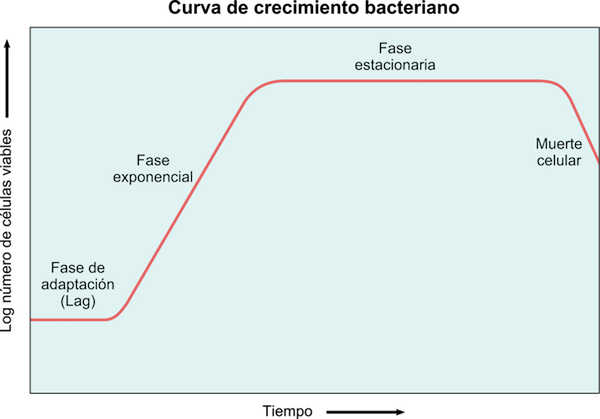
\includegraphics[width=0.85\linewidth]{07_curva_de_crecimiento_microbiano}
    \caption{Ejemplo de curva de crecimiento microbiano}
    \label{fig:curva_crecimiento_microbiano}
\end{figure}

\begin{figure}[H]
    \centering
    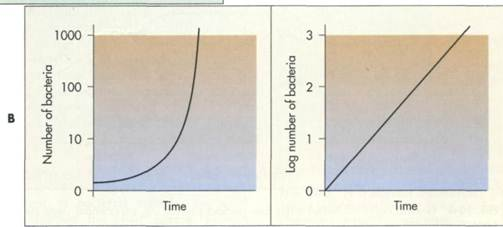
\includegraphics[width=0.85\linewidth]{07_crecimiento_microbiano_log}
    \caption{Diferencia entre gráfica con número directo de bacterias y gráfica con escala logarítmica}
    \label{fig:crecimiento_microbiano_log}
\end{figure}

Los microorganismos presentan un crecimiento exponencial, que puede representarse con $2^{n}$, siendo $n$ el número de divisiones o generaciones dadas. Con esto en cuenta, para calcular una población solo necesitaríamos calcular $N_{0} \cdot 2^{n}$, siendo $N_{0}$ la población inicial.

Estos datos pueden graficarse de manera directa y se obtendría una linea exponencial, tal como se ve en la \autoref{fig:crecimiento_microbiano_log} sin embargo, puede resultar mejor aplicarles un logaritmo para obtener una linea recta, que puede ser estudiada con la respectiva ecuación de la recta ($y=mx+b$).

Algo a tener en cuenta es que distintas poblaciones presentan a su vez distintos tiempos de duplicación o generación, valor que se representa como $t_{d}$, y este se ve afectado por las condiciones del medio (sustrato, temperatura, pH, etcétera).

Es posible obtener el número de generación en la que un cultivo dado se encuentra a partir de la magnitud de las poblaciones, esto mediante un pequeño despeje de la fórmula anteriormente descrita:

\begin{equation*}
    N_{t} = N_{0} \cdot 2^{n} \longrightarrow n = \frac{\log{(N_{t})} - \log(N_{0})}{\log(2)}
\end{equation*}

Dado que la cinética estudia el cambio, a la cinética de crecimiento microbiano le interesa saber el ritmo a la que un cultivo dado crece en distintos puntos del tiempo. El cambio en la cantidad de biomasa puede representarse con la siguiente ecuación:

\begin{equation*}
    r_{x} = \mu x
\end{equation*}

Esto también podemos expresarlo como una ecuación diferencial de la siguiente manera:

\begin{equation*}
    \frac{dx}{dt} = \mu x
\end{equation*}

Esta nos dice cuanto cambia la cantidad de biomasa ($x$) respecto al tiempo ($t$). A su vez, $\mu$ es la velocidad específica a la que se da ese crecimiento microbiano. El cálculo de $\mu$ es posible resolviendo tal ecuación diferencial.

\begin{align*}
    \frac{dx}{dt} &= \mu x
    \\
    \\
    \frac{1}{x} \ dx &= \mu \ dt
    \\
    \\
    \int_{x_{0}}^{x}{\frac{1}{x}} \ dx &= \int_{t_{0}}^{t_{d}}{\mu \ dt}
    \\
    \\
    \ln(x) - \ln(x_{0}) &= \mu \cdot (t_{d} - 0)
    \\
    \\
    \mu &= \frac{\ln(x) - \ln(x_{0})}{t}
\end{align*}